\documentclass[a4paper,12pt]{article}
\usepackage{amssymb} %\mathbb
\usepackage{amsmath} % {align}
\usepackage{xcolor}
\usepackage{verbatim}
\usepackage{listings}
\usepackage{multirow}
\usepackage{graphicx}
\usepackage{hyperref}
\hypersetup{
    colorlinks=true,
    linkcolor=blue,
    filecolor=magenta,      
    urlcolor=cyan,
    pdftitle={ECE655\_Project\_3},
    pdfpagemode=FullScreen,
    }
\usepackage{subcaption}
\usepackage{wrapfig}
%\usepackage[most]{tcolorbox}
\usepackage[utf8]{inputenc}
\usepackage[english]{babel}
\usepackage{booktabs}
\usepackage{mdframed}
\usepackage{makecell}
\usepackage{array}
\usepackage{pbox}
\usepackage{textcomp}
\usepackage{upgreek}
\usepackage{gensymb}
\usepackage{longtable}
\usepackage{enumerate}
\usepackage{enumitem}
\usepackage{booktabs} % To thicken table lines
\usepackage{hyphenat}
\usepackage{url}
\usepackage{hyperref}

\definecolor{codegreen}{rgb}{0,0.6,0}
\definecolor{codegray}{rgb}{0.5,0.5,0.5}
\definecolor{codepurple}{rgb}{0.58,0,0.82}
\definecolor{backcolour}{rgb}{0.95,0.95,0.92}
\definecolor{filename}{rgb}{0.1,0.1,0.99}
\definecolor{textout}{rgb}{0.3,0.4,0.3}

\newcommand{\purple}[1]{\textsf{\textcolor{codepurple}{#1}}}

\lstdefinestyle{mystyle}{
    backgroundcolor=\color{backcolour},   
    commentstyle=\color{codegreen},
    keywordstyle=\color{magenta},
    numberstyle=\tiny\color{codegray},
    stringstyle=\color{codepurple},
    basicstyle=\ttfamily\footnotesize,
    breakatwhitespace=false,         
    breaklines=true,                 
    captionpos=b,                    
    keepspaces=true,                 
    numbers=left,                    
    numbersep=5pt,                  
    showspaces=false,                
    showstringspaces=false,
    showtabs=false,                  
    tabsize=2
}

\lstset{style=mystyle}

%\renewcommand{\texttt}[1]{%
%  \begingroup
%   \ttfamily
%   \begingroup\lccode`~=`/\lowercase{\endgroup\def~}{/\discretionary{}{}{}}%
%   \begingroup\lccode`~=`[\lowercase{\endgroup\def~}{[\discretionary{}{}{}}%
%   \begingroup\lccode`~=`.\lowercase{\endgroup\def~}{.\discretionary{}{}{}}%
%   \catcode`/=\active\catcode`[=\active\catcode`.=\active
%   \scantokens{#1\noexpand}%
%   \endgroup
% }

% Define todo                                                                   
\newcommand{\TODO}[1]{\textcolor{red}{[TODO: #1]}}
\newcommand{\ans}[1]{\textcolor{blue}{\textbf{#1}}}

\newcommand{\FILE}[1]{\textsf{\textcolor{filename}{#1.py}}}
\newcommand{\FILe}[1]{\textsf{\textcolor{filename}{#1}}}
\newcommand{\lst}[1]{ \vspace{10pt}\lstinputlisting[language=Python]}
\newcommand{\LST}[1]{ \vspace{10pt}\lstinputlisting[language=Python,caption=\textsf{\textcolor{filename}{#1.py}}]{code/#1.py}}
\newcommand{\ou}[1]{\begin{itemize}\item[]\textsf{\small\textcolor{textout}{#1}}\end{itemize}}
\newcommand{\OU}[1]{ \vspace{-8pt}\noindent\rule{\textwidth}{1pt}\vspace{-12pt}\begin{itemize}\item[]\textsf{\footnotesize\textcolor{textout}{#1}}\end{itemize}\vspace{-16pt}\rule{\textwidth}{1pt}}
\newcommand{\out}[1]{ \noindent\rule{\textwidth}{1pt}\vspace{-24pt}\begin{itemize}\item[]\textsf{\textcolor{textout}{#1}}\end{itemize}\vspace{-28pt}\rule{\textwidth}{1pt}}
\newcommand{\Out}[1]{ \noindent\rule{\textwidth}{1pt}\vspace{-24pt}\begin{itemize}\item[]\textsf{\textcolor{textout}{#1}}\end{itemize}\vspace{-18pt}\rule{\textwidth}{1pt}}
\newcommand{\OUt}[1]{ \noindent\rule{\textwidth}{1pt}\vspace{-12pt}\begin{itemize}\item[]\textsf{\textcolor{textout}{#1}}\end{itemize}\vspace{-18pt}\rule{\textwidth}{1pt}}
\newcommand{\OUT}[1]{ \noindent\rule{\textwidth}{1pt}\vspace{-10pt}\begin{itemize}\item[]\textsf{\textcolor{textout}{#1}}\end{itemize}\vspace{-10pt}\rule{\textwidth}{1pt}}
%\newcommand{\OUT}[1]{ \rule{\textwidth}{1pt}\vspace{2pt}\textsf{\textcolor{textout}{#1}}\rule{\textwidth}{1pt}}
\newcommand{\CMD}[1]{\textsf{\textcolor{magenta}{#1}()}}
\newcommand{\CMd}[1]{\textsf{\textcolor{magenta}{#1}}}
\newcommand{\cmd}[1]{\textsf{\small\textcolor{magenta}{#1}()}}
\newcommand{\VAR}[1]{\textsf{\textbf{#1}}}
\newcommand{\TYPE}[1]{\textbf{\emph{#1}}}
\newcommand{\VSEP}{\vspace{4pt}\noindent}
\newcommand{\HSEP}{\hspace{10pt}}
\newcommand{\PY}[1]{\lstinline[language=Python]{#1}}
\newcommand{\PYout}[1]{\textsf{\textcolor{textout}{#1}}}
\newcommand{\SP}{\textvisiblespace}
\newcommand{\SPP}{\textvisiblespace\textvisiblespace}
\newcommand{\SPPP}{\textvisiblespace\textvisiblespace\textvisiblespace}
\newcommand{\SPPPP}{\textvisiblespace\textvisiblespace\textvisiblespace\textvisiblespace}
\newcommand{\ERROR}[1]{\textcolor{red}{\small #1}}
\newcommand{\Error}[1]{\textcolor{red}{\footnotesize #1}}

\newcommand{\specialcell}[2][c]{%
\begin{tabular}[#1]{@{}c@{}}#2\end{tabular}}


\begin{document}
 \title{ECE655 Project 03\\
                \vspace{4pt}
                \small{Author: Stewart Schuler}
                \vspace{-12pt}}
 \date{}
 \maketitle
 \begin{center}
 \textbf{Due: 10/12/2025}
 \end{center}

\tableofcontents
\newpage
\section{Part A}
\label{sec:sec_a}
The dataset chosen for this project compares the mean global sea level per year. That data is sourced from the \textit{University of Colorado}\footnote{\url{https://sealevel.colorado.edu/data/2020rel1-0}}.


\begin{figure}[htpb]
	\centering
	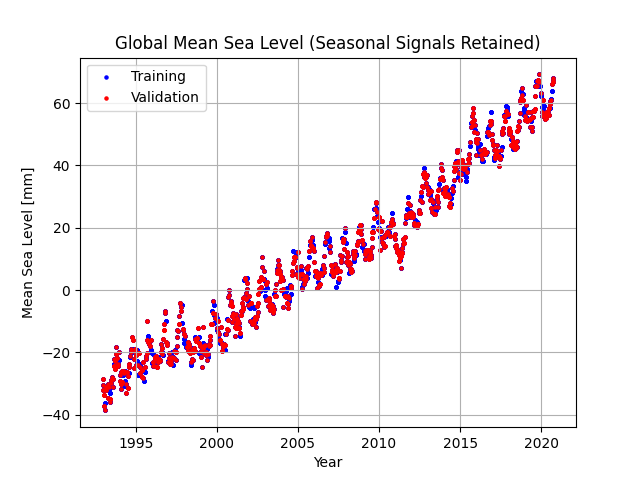
\includegraphics[width=\columnwidth]{figures/dataset.png}
	\label{fig:part_a}
\end{figure}

It can be seen there is a clear linear trend between year and mean sea level. The dataset was then partitioned into an 80/20 split of training and validation data. Applying linear regression to the (normalized) training data learned a line with an $b=0.9758$ and $w=0.9758$.

\LST{part\_a}

\begin{figure}[htpb]
	\centering
	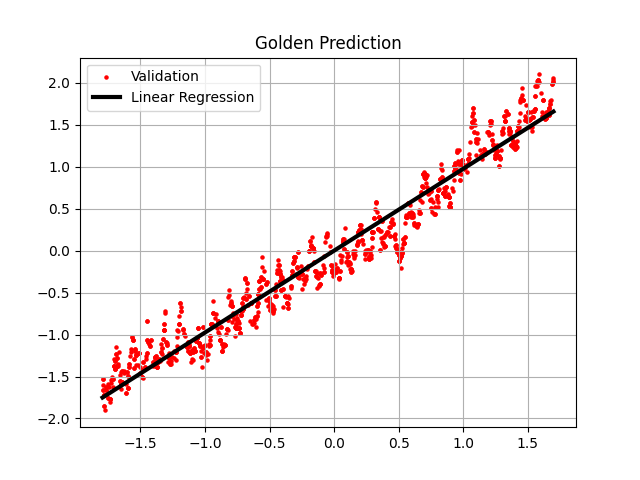
\includegraphics[width=\columnwidth]{figures/linear_regression.png}
	\label{fig:part_a}
\end{figure}

The regression line was found to have a MSE of $0.0489$
\newpage
\section{Part B}
\label{sec:sec_b}
A loss surface was created by computing the MSE for a grid of $10,000$ \textit{b} and \textit{w} pairs. Both variables were varied by $\pm3$ from the golden value found in Section~\ref{sec:sec_a}.

\begin{figure}[htpb]
	\centering
	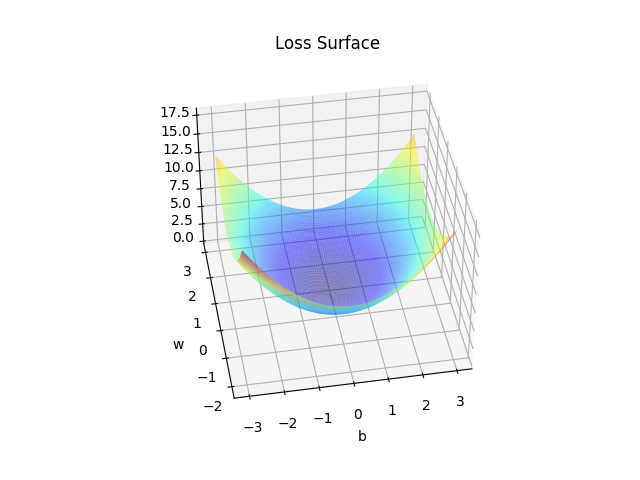
\includegraphics[width=\columnwidth]{figures/loss_surface.png}
	\label{fig:loss_surface}
\end{figure}

The above surface was generated using the following code.
\LST{part\_b}
\newpage
\section{Part C}
\label{sec:sec_c}

Next, because we are using linear regression the dataset must be made linear. In order to do so, the natural log was taken of \textit{I}$_{d}$. Linear regression was than ran by manually computing the gradients as shown in the below code. Training lasted for $500$ epochs and has a learning rate of $0.01$. MSE was used to compute the loss and the loss curve is shown in Figure~\ref{fig:loss}. After training the final value of \textit{b} and \textit{w} were found to be $-15.2738$ and $15.5091$ respectively when unnormalized. The training loss for the final epoch was $0.001532$

\LST{part\_c}

\begin{figure}[!htpb]
	\centering
	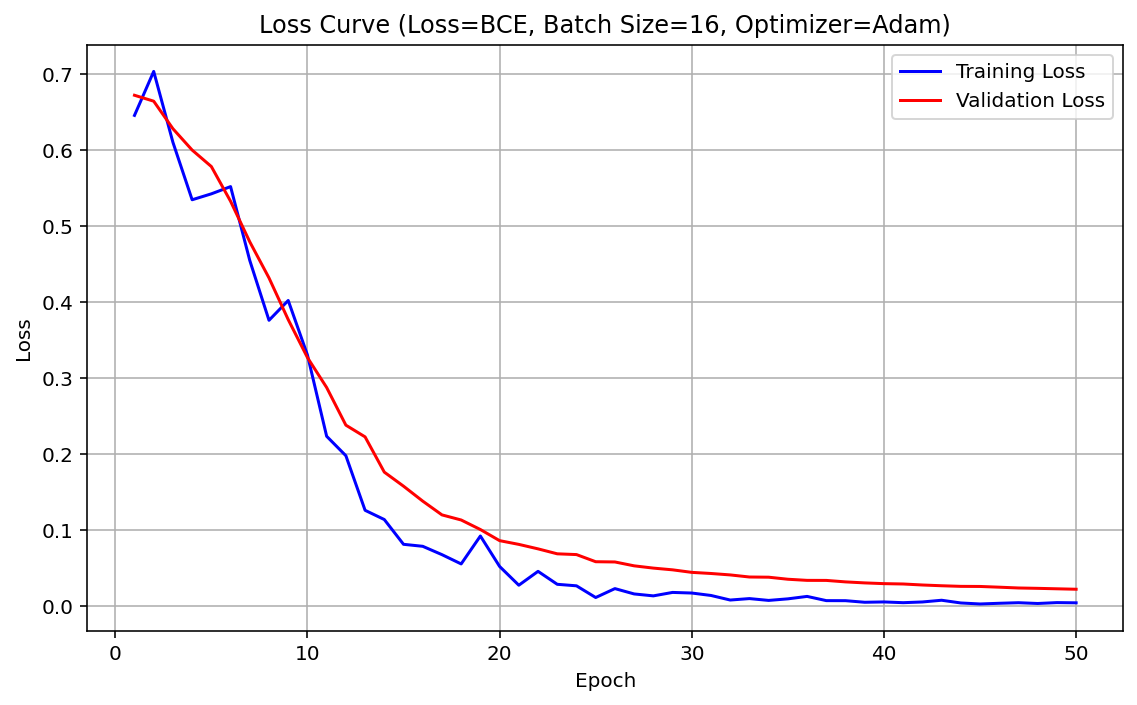
\includegraphics{figures/loss.png}
	\caption{Training Loss Curve}
	\label{fig:loss}
\end{figure}
\newpage
\section{Part D}
\label{sec:sec_d}
Next to consider the impact of changing the optimizer the loss was set back to \textbf{MSE} loss and the optimizer was changed to \textbf{Adam}. 

\LST{part\_d}

It can be seen in Figure~\ref{fig:d loss} that the curve mains it's exponential shape that it had when using the \textbf{SGD} optimizer but it is approaching convergence much slower.
\begin{figure}[htpb]
	\centering
	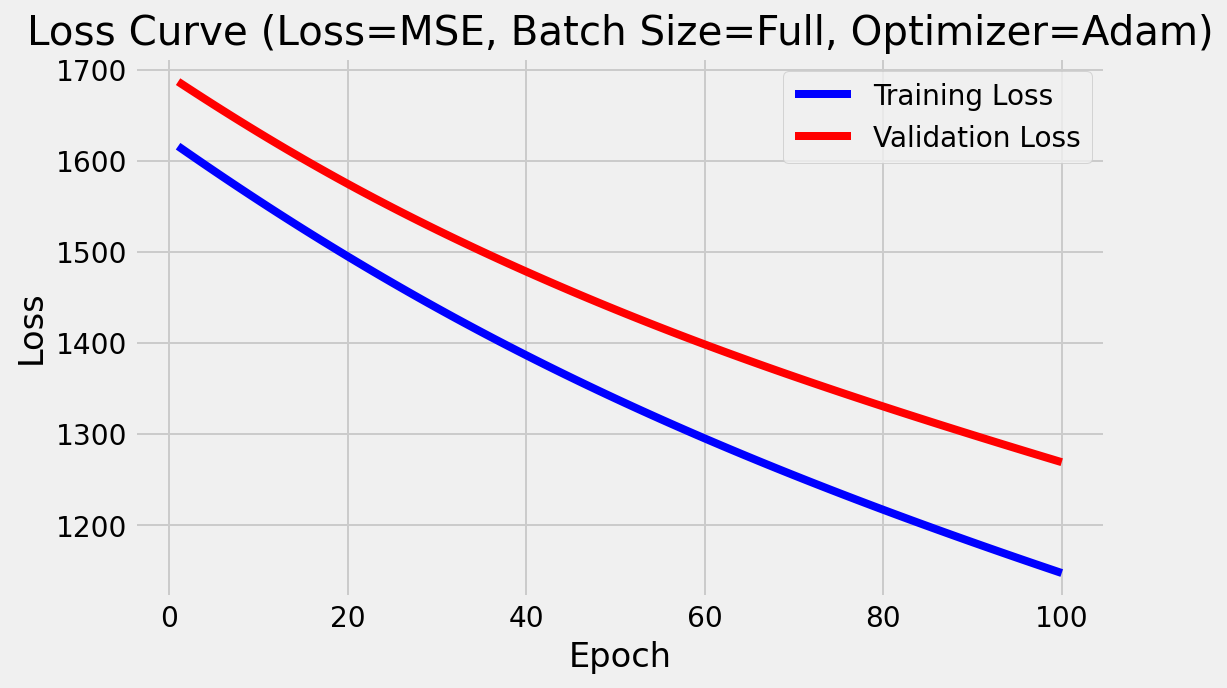
\includegraphics[width=\columnwidth]{figures/d_loss.png}
	\caption{Loss Curve with (\textbf{Adam}, \textbf{MSE}, \textbf{full})}
	\label{fig:d loss}
\end{figure}



\newpage
\section{Part E}
\label{sec:sec_e}

In this experiment we consider how changing the batch size impacts the training. 

\LST{part\_e}

It can be seen in Figure~\ref{fig:e loss} that the final training and validations losses are not the same depending on the batch sizes. For this specific dataset with 331 training samples after the split a batch size of 16 produced the best final loss values.
\begin{figure}[htpb]
	\centering
	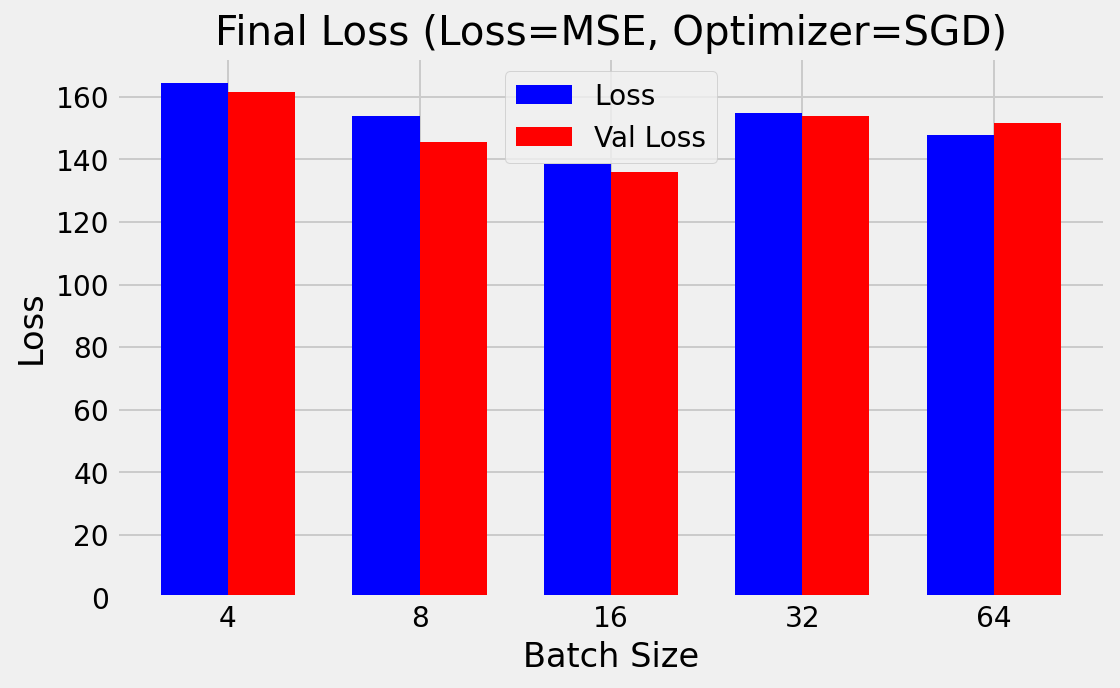
\includegraphics[width=\columnwidth]{figures/e_loss.png}
	\caption{Fianl Losses with (\textbf{SGD}, \textbf{MSE}, \textbf{Variable Batch Size})}
	\label{fig:e loss}
\end{figure}
\newpage
\section{Part F}
\label{sec:sec_f}

In this experiment we sweep two different optimizers (\textbf{Adam} and \textbf{SGD}) across different number of training epochs. Figure~\ref{fig:f} compares the final training loss after $X$ epochs and the training time. For this experiment training was ran entirely on the CPU.

\LST{part\_f}

It can be seen that with a large number of Epochs the \textit{Adam} optimizer does eventually converge towards the same values as the \textit{SGD} optimizer. And the ADAM runtime is slightly slower.

\begin{figure}[htpb]
	\centering
	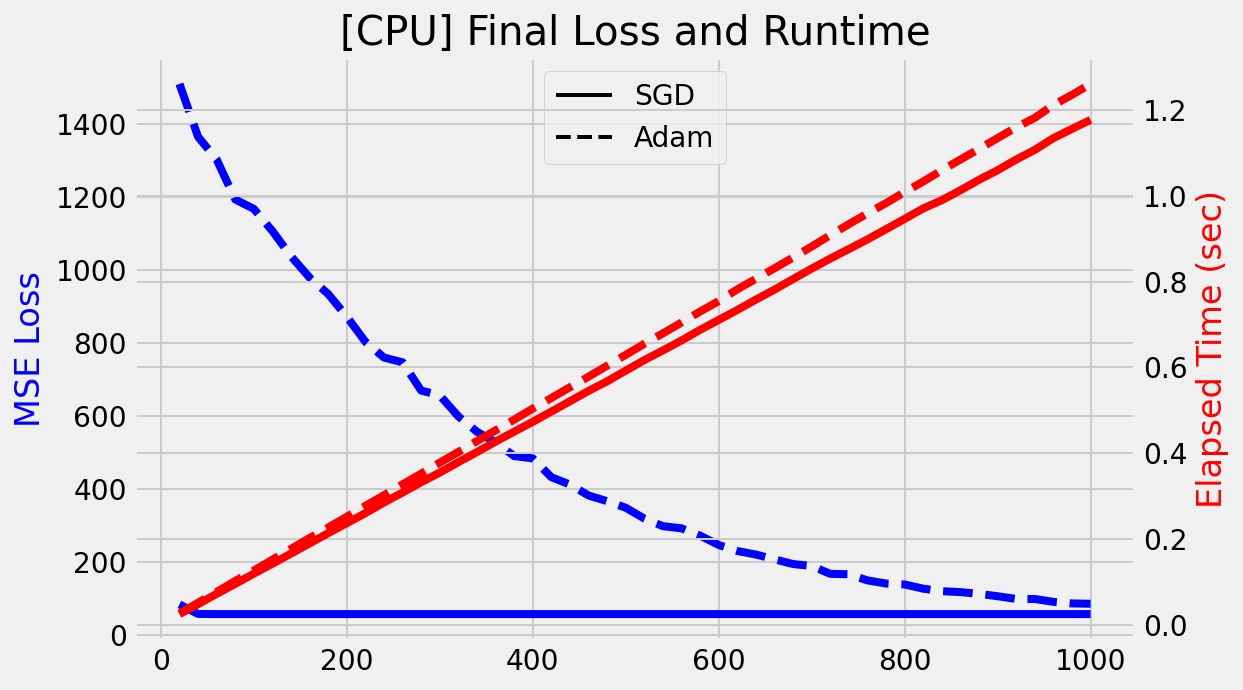
\includegraphics[width=\columnwidth]{figures/cpu_timing.png}
	\caption{CPU Final Training loss and Runtime vs Epochs}
	\label{fig:f}
\end{figure}



\newpage
\section{Part G}
\label{sec:sec_g}

The same experiment from the previous section was reran, with the modification of targeting the GPU. The hardware being tested on was an \textit{AMD 7900 GRE} using \textit{ROCm} support for \textit{pytorch}.

\LST{part\_g}

Surprisingly, as shown in Figure~\ref{fig:g}, when processing on the GPU the comparable runtimes were actually slower than on the CPU. This result is likely because the dataset is so small that the overhead associated with moving the data to/from the GPU and launching the kernels negates any performance improvements that come from processing on the GPU. Also since the Linear Regression model is only a single (6,1) neuron there isn't mass parallelization available for each parameter like there would be in a deep model. Additionally the ROCm framework is not as well optimized as the CUDA based implementations.

\begin{figure}[htpb]
	\centering
	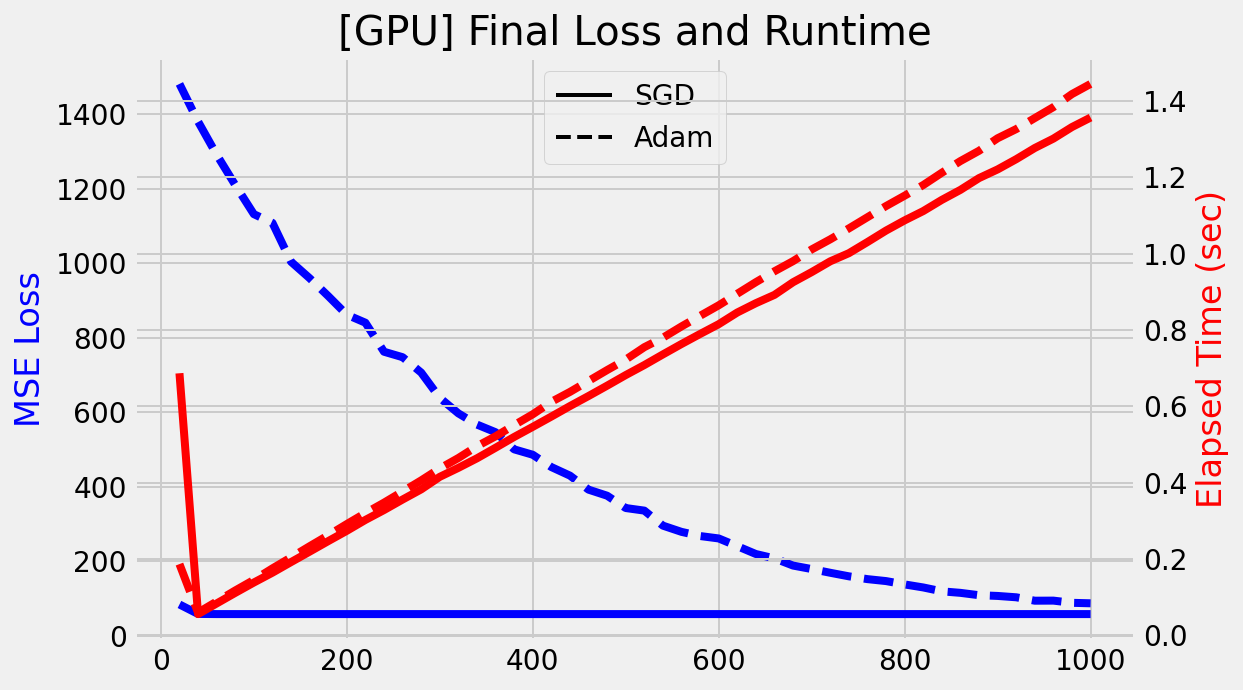
\includegraphics[width=\columnwidth]{figures/gpu_timing.png}
	\caption{GPU Final Training loss and Runtime vs Epochs}
	\label{fig:g}
\end{figure}

Out of curiosity I tried to see if I could demonstrate a significant GPU performance increase. To address the small dataset problem I created a $1,000,000$ point 50 feature data dataset with a trivial noise linear model. Figure~\ref{fig:g speedup} shows the final runtime for training it with the CPU and GPU. It can be seen that my GPU did improve performance by roughly a factor of 4. Meaning in the above experiment, had the dataset been larger the runtimes would've been improved.  

\begin{figure}[htpb]
	\centering
	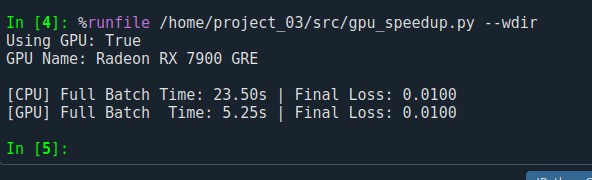
\includegraphics[width=\columnwidth]{figures/gpu_speedup.png}
	\caption{GPU Performance Increase}
	\label{fig:g speedup}
\end{figure}



\end{document}

